\section{Herramientas de soporte a la creacion de modelos de software}

\begin{spacing}{4.0}
\end{spacing}
\subsection{Una arquitectura de dos niveles: modelo vs. metamodelos}
\begin{spacing}{2.0}
\end{spacing}
Los lenguajes de modelado visuales son lenguajes gráficos que se usan para la especificación,
visualización, documentación de productos de software como paso previo a su construcción.
Generalmente el marco conceptual de las notaciones de modelado se basa sobre una arquitectura
formada por distintos niveles (ver figura 5 [Odell95]). La descripción de esta arquitectura puede
encontrarse por ejemplo en [UML 97b].
\\\\
\begin{figure}[H]
\centering
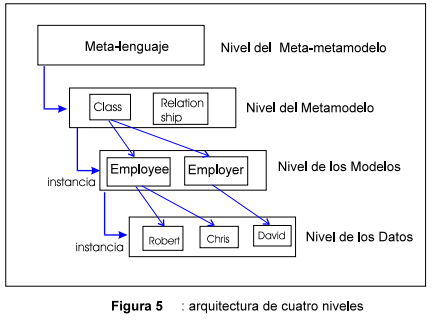
\includegraphics[scale=0.5]{./Imagenes/modelo19}
\caption{Ejemplo de figura 1-2}
\label{figura1}
\end{figure}
\subsection{Existen dos niveles principales:}
\begin{spacing}{2.0}
\end{spacing}
\textbf{1. El nivel del metamodelo:}
\begin{spacing}{2.0}
\end{spacing}
El metamodelo es un modelo para la información que puede ser
expresada durante la construcción del modelo de un sistema. Básicamente, define los
elementos de modelado tales como Class diagrams, State machines, Sequence diagrams
en el metamodelo de UML. Además define en que forma estos elementos se relacionan para
conformar el modelo de un sistema. El metamodelo es una descripción del lenguaje de
modelado en sí. Su semántica es el conjunto de todos los modelos bien formados. El
metamodelo es independiente de cualquier modelo en particular, él describe los elementos
del lenguaje y las restricciones que deben cumplir todos los modelos, por ejemplo: “dentro
de un Classifier los nombres de los atributos no se repiten”
\begin{spacing}{2.0}
\end{spacing}

\textbf{2. El nivel del modelo:}
\begin{spacing}{2.0}
\end{spacing}
Por otro lado, el modelo es una instancia del metamodelo. El modelo
(en realidad un modelo no es una unidad sino que es un conjunto de diversos modelos
relacionados, tal como fue explicado en la sección 1.3) describe los objetos inherentes al
dominio de la aplicación que está siendo modelada, por ejemplo: Employer, Employee,
BankAccount, Client, etc. e incluye restricciones que deben ser satisfechas por los objetos
del sistema, por ejemplo “no se permiten extracciones cuando el saldo de una cuenta es
menor que cero”
\begin{spacing}{2.0}
\end{spacing}
\subsection{Existen además otros dos niveles relacionados con los anteriores:}
\begin{spacing}{2.0}
\end{spacing}

\textbf{1. El nivel de los datos:}
\begin{spacing}{2.0}
\end{spacing}
 En el nivel de los datos, las entidades son instancias de las clases del
modelo, por ejemplo los objetos Robert y Chris son instancias de la Clase Employee.
\begin{spacing}{2.0}
\end{spacing}
\textbf{2. El nivel del meta-metamodelo:}
\begin{spacing}{2.0}
\end{spacing}
Es necesario contar con un nivel superior describiendo el
lenguaje utilizado para expresar el metamodelo. Este nivel superior es llamado metametamodelo. Por ejemplo en esta tesis utilizaremos Dynamic Logic como meta-lenguaje.

\subsection{Herramientas de metamodelado}
\begin{spacing}{2.0}
\end{spacing}
Herramientas de metamodelado. Son las herramientas básicas para diseñar el metamodelo de acuerdo al lenguaje de metamodelado, tal como se plantea en (Gómez y Sánchez, 2006).

\subsection{Ventajas}
\begin{spacing}{2.0}
\end{spacing}

Según (Quasar Tecnología, 2007) la aplicación de herramientas de metamodelado en una entidad o proyecto puede traer consigo varias ventajas, entre las que se encuentran

\begin{spacing}{2.0}
\end{spacing}

\begin{itemize}
    \item Reducción en tiempo y recursos para el mantenimiento de las aplicaciones existentes.

Todo desarrollador de software sabe que los productos que realizan, por representar modelos de lo que ocurre en el mundo real, son cambiantes y dinámicos, por lo que deben ser adaptables a las nuevas exigencias de los clientes o beneficiarios institucionales, esto conlleva a realizar un proceso que involucra grandes cambios. La aplicación del metamodelado, implica que los pasos a seguir para realizar la misma modificación sean menores. Este cambio en el paradigma del mantenimiento de las aplicaciones genera sustanciales beneficios a la organización que toma la decisión de adoptar esta tecnología para la construcción y mantenimiento de sus sistemas de información.

    \item Evita la introducción de errores en los programas.

La capacidad de introducir una nueva funcionalidad en un sistema de información sin escribir líneas de código adicional, elimina la posibilidad de introducir errores de programación cuyo costo tanto para la información registrada (errores en la base de datos a causa de un programa erróneo) o el costo de ubicar, corregir y probar el código fuente causante del error, son eliminados.

    \item Reducción en el tiempo de entrenamiento a los usuarios.

Luego de entrenar un usuario en la utilización de estas herramientas, el entrenamiento para que aprenda a utilizar la aplicación del metamodelo para otras aplicaciones, se reduce a trabajar con éste sobre los formatos, grupos y campos de información con los cuales se ha estructurado la información en el nuevo contexto. Esto gracias a la unicidad de las interfaces en el software de registro y consulta de información.

    \item Generación de consultas a la medida.

El sistema generador de consultas para un metamodelo, se convierte en una herramienta muy poderosa en manos de las personas que dominan el contexto temático de la información registrada en este metamodelo, ya que puede consultar, ordenar, agrupar, graficar o producir información alfanumérica para la información registrada

\end{itemize}

\subsection{AToM3}
\begin{spacing}{2.0}
\end{spacing}

A Tool for Multi-Formalism Modelling and Meta-Modelling (AToM3) es una herramienta MetaCASE escrita en el lenguaje de programación Python, y está enfocada a los flujos de trabajo de Análisis y Diseño. Posee un procesador que incluye un meta-metamodelo inicial basado en el modelo entidad-relación, que permite la definición de los diferentes metamodelos en un entorno gráfico con las mismas características que emplea el usuario en la construcción de los diferentes modelos. De esta manera, se puede definir cualquier tipo de metamodelo en términos de las entidades que forman parte del mismo y sus posibles interconexiones o relaciones. Una vez definido el metamodelo, se puede emplear su definición para construir los modelos pertinentes a un problema específico del mundo.(Zapata y Álvarez, 2005)

AToM3 tiene la posibilidad de expresar restricciones en términos de gramáticas de grafos incorporadas a su entorno. Las gramáticas de grafos tienen similitudes con las gramáticas basadas en texto en el sentido de que pueden ser usadas para describir las transformaciones a un grafo determinado; la diferencia radica en que las reglas de ese tipo de gramáticas se expresan de manera gráfica y no a modo de texto.

Las gramáticas de grafos se definen como un conjunto de reglas que poseen un lado izquierdo (LHS, por sus siglas en inglés, left-hand side) que contiene las precondiciones (expresadas de forma gráfica) que deben ser cumplidas para activar una determinada regla y un lado derecho (RHS, por sus siglas en inglés, right-hand side) que contiene el grafo que remplazará el que equivale al lado izquierdo de la regla.

Para las reglas expresadas de esta manera se deben definir condiciones y acciones para ejecutar cuando la regla se active. La gramática de grafos de AToM3 posee también un mecanismo que va reescribiendo el modelo a medida que las diferentes reglas se van activando hasta que no haya reglas que se puedan ejecutar. (Zapata y Álvarez, 2005)

\begin{spacing}{2.0}
\end{spacing}

\subsection{AndroMDA}
\begin{spacing}{2.0}
\end{spacing}

AndroMDA (pronunciado “Andrómeda”) es una herramienta de metamodelado escrita en el lenguaje Java bajo la licencia Berkeley Software Distribution (BSD), que está enfocada a todo el proceso de desarrollo de software. Es un programa informático de tipo framework. Se considera un motor de transformación de modelos en código fuente.

AndroMDA convierte modelos de algunas herramientas de modelado UML en componentes listos para su despliegue en un gran número de lenguajes entre los que se encuentran Java, PHP, .NET, HTML, sólo con utilizar los cartuchos adecuados.

Estos cartuchos dirigen el desarrollo de aplicaciones basadas en componentes y son fundamentales para el proceso de generación de código. La herramienta permite la creación de mecanismos para la construcción de nuevos cartuchos. (AndroMDA, 2006)

\begin{spacing}{2.0}
\end{spacing}

\
